%&preamble
% automatic hyphenation for 2 languages
% http://www.mechpedia.gr/wiki/Hyphenation_-_%CE%A5%CF%86%CE%B5%CE%BD%CF%8E%CF%83%CE%B5%CE%B9%CF%82#.CE.91.CF.85.CF.84.CF.8C.CE.BC.CE.B1.CF.84.CE.B5.CF.82_.CF.85.CF.86.CE.B5.CE.BD.CF.8E.CF.83.CE.B5.CE.B9.CF.82_.CF.83.CE.B5_.CE.B4.CE.AF.CE.B3.CE.BB.CF.89.CF.83.CF.83.CE.B1_.CE.BA.CE.B5.CE.AF.CE.BC.CE.B5.CE.BD.CE.B1
% very slow, enable only at final pdf.
%\usepackage[Greek,Latin]{ucharclasses}
%\setTransitionsForGreek{\selectlanguage{greek}}{\selectlanguage{english}}

% polyglossia
\usepackage{polyglossia}
\setmainlanguage{greek}
\setotherlanguages{english}

% Fonts
% fonts can't go in the .fmt file
\usepackage{fontspec}
\setmainfont[Mapping=tex-text]{DejaVu Sans}
\newfontfamily\greekfont[Script=Greek]{DejaVu Sans}
\newfontfamily\greekfontsf[Script=Greek]{DejaVu Sans}
\setmonofont{Hack}
\newfontfamily\greekfonttt[Scale=1.0]{Hack}
\usepackage{microtype} % microtype is font-dependant


\title{%
  \vspace{0.3cm}%
  \hrule height 2pt%
  \vspace{0.3cm} Δίκτυα Υπολογιστών ΙΙ\\
  Εργασία Δικτυακού Προγραμματισμού%
  \vspace{0.3cm}%
  \hrule height 2pt%
  \vspace{0.3cm}
}

\author{%
  Φλώρος-Μαλιβίτσης Ορέστης, 7796  \href{mailto:orestisf@ece.auth.gr}{orestisf@ece.auth.gr}\\
  \textbf{Τομέας Ηλεκτρονικής}\\
  \textbf{Τμήμα Ηλ. Μηχανικών / Μηχανικών ΗΥ}\\
  \textbf{Αριστοτέλειο Πανεπιστήμιο Θεσσαλονίκης}
}
\titlepic{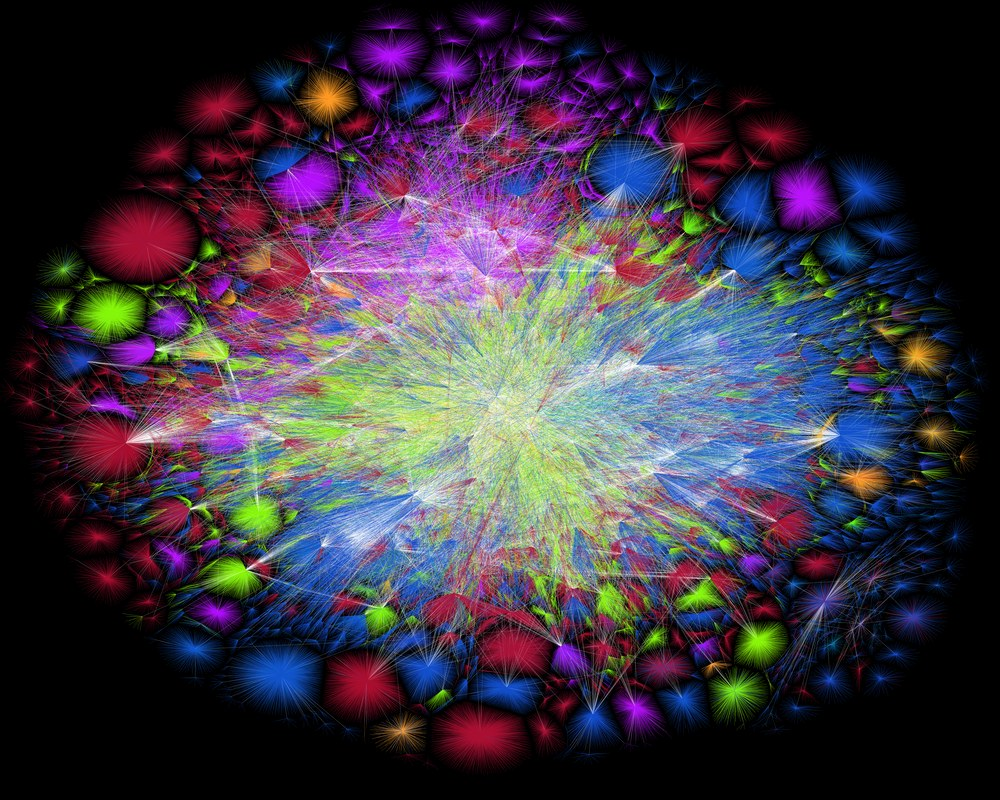
\includegraphics[width=\linewidth]{images/cover}}

% Variables & constants definitions:
\newcommand{\appname}{\texttt{userApplication}}
\newcommand{\scriptname}{\texttt{extract-codes.py}}

\begin{document}
\pagenumbering{roman}
\deactivateBG
\maketitle
\tableofcontents
\listoflistings
\listoffigures
\listoftables
\clearpage % Ensure background starts after this.
% Chapters start from here on:
\activateBG
\pagenumbering{arabic}
\setcounter{page}{1}

\section{Εισαγωγή}
Αφορά την \sessionnumber{} σύνοδο με την Ιθάκη.
Η σύνοδος αυτή άρχισε στις \sessiondatestart{} και τελείωσε στις \sessiondateend{}.
Οι παράμετροι που χρησιμοποιήθηκαν φαίνονται στον πίνακα
\hyperref[table:codes]{\ref{table:codes}}.

\begin{table}
\centering
\begin{tabular}{c|c}
\hline
\multicolumn{1}{c}{\bfseries Παράμετρος} & \multicolumn{1}{|c}{\bfseries Τιμή}\\\hline
Client Address&\clientaddress{}\\
Client Listening Port&\clientlisteningport{}\\
Server Listening Port&\serverlisteningport{}\\
Echo Request Code&\echorequestcode{}\\
Image Request Code&\imagerequestcode{}\\
Sound Request Code&\soundrequestcode{}\\
\end{tabular}
\caption{Παράμετροι για την \sessionnumber{} σύνοδο}
\label{table:codes}
\end{table}
\FloatBarrier

\chapter{Βιβλιογραφική αναφορά}
\section{Το πρωτόκολλο UDP}
Το πρωτόκολλο UDP (User Datagram Protocol ή Universal Datagram Protocol)
είναι ένα από τα βασικά πρωτόκολλα που χρησιμοποιούνται στο Internet.
Σχεδιάστηκε το 1980 και ορίζεται στο RFC 768\cite{rfc768}\cite{wiki:udp}.

Αποτελεί ένα απλό,
\href{https://en.wikipedia.org/wiki/Connectionless_communication}{connectionless}
πρωτόκολλο στο οποίο δεν υπάρχουν διάλογοι
\href{https://en.wikipedia.org/wiki/Handshaking}{"handshaking"}.
Δηλαδή, η επικοινωνία μέσω του UDP δεν προσφέρει την δυνατότητα στις συνδεδεμένες συσκευές να "θυμούνται" που βρίσκονται σε μια "συνομιλία" ανταλλαγής μηνυμάτων.
Η επικοινωνία γίνεται μέσω σύντομων μηνυμάτων (γνωστών και ως
\href{https://en.wikipedia.org/wiki/Datagram}{datagrams}
) από τον έναν υπολογιστή στον άλλον μέσα σε ένα δίκτυο υπολογιστών.

Ένα από τα κύρια χαρακτηριστικά του UDP είναι ότι δεν εγγυάται αξιόπιστη επικοινωνία.
Τα πακέτα UDP που αποστέλλονται από έναν υπολογιστή μπορεί να φτάσουν στον παραλήπτη με λάθος σειρά, διπλά ή να μην φτάσουν καθόλου ανάλογα με την τρέχουσα κατάσταση του δικτύου.
Αντιθέτως, το πρωτόκολλο
\href{https://en.wikipedia.org/wiki/Transmission_Control_Protocol}{TCP}
διαθέτει όλους τους απαραίτητους μηχανισμούς ελέγχου και επιβολής της αξιοπιστίας και μπορεί να εγγυηθεί την αξιόπιστη επικοινωνία μεταξύ των υπολογιστών.
Ωστόσο, λόγω της έλλειψης των μηχανισμών αυτών, το πρωτόκολλο UDP καθιστάται αρκετά πιο γρήγορο και αποτελεσματικό

%TODO: section with router settings.
\newcommand{\codeRef}[1]{\hyperref[section:#1]{\mintinline{java}!#1()!}}
\chapter{Η εφαρμογή (\appname{})}
\section{Script \scriptname{}}
Για την γρήγορη εξαγωγή των κωδικών από το site \url{http://ithaki.eng.auth.gr/netlab/index.html} γράφτηκε ένα script σε
\href{https://www.python.org/}{python3}
όπου πραγματοποιεί τη σύνδεση (login) με το site με τα σχετικά credentials και εξάγει σε ένα αρχείο τους κωδικούς σε μορφή
\href{https://en.wikipedia.org/wiki/JSON}{json} ώστε να μπορούν εύκολα να διαβαστούν οι τελευταίοι κωδικοί αυτόματα από την εφαρμογή \appname{}.
Χρησιμοποιήθηκαν οι εξωτερικές βιβλιοθήκες:
\begin{itemize}
\item \href{http://docs.python-requests.org/en/master/}{requests} για την πραγματοποίηση της συνεδρίας, και το downloading των σχετικών σελίδων.
\item \href{http://www.crummy.com/software/BeautifulSoup/}{BeautifulSoup} για το parsing των \texttt{.html} αρχείων για την εξαγωγή των κωδικών.
\end{itemize}

Καθώς δεν είναι δυνατό το ανέβασμα επιπλέον αρχείου με το όνομα \scriptname{} ο κώδικας παρατίθεται εδώ:
\begin{code}
\inputminted[frame=single, breaklines=true, linenos=true, python3=true]{python}{../extract-codes.py}
\caption{Το script \scriptname{}}
\label{listing:extract-codes}
\end{code}

\section{Χρήση βιβλιοθηκών \& imports}
\begin{code}
\begin{minted}{java}
import com.google.gson.Gson;
import com.google.gson.JsonObject;
import com.google.gson.stream.JsonReader;

import javax.sound.sampled.AudioFormat;
import javax.sound.sampled.AudioSystem;
import javax.sound.sampled.LineUnavailableException;
import javax.sound.sampled.SourceDataLine;
import java.io.*;
import java.net.*;
import java.nio.ByteBuffer;
import java.nio.ByteOrder;
import java.util.Arrays;
import java.util.logging.ConsoleHandler;
import java.util.logging.Handler;
import java.util.logging.Level;
import java.util.logging.Logger;

import static javax.xml.bind.DatatypeConverter.printHexBinary;
\end{minted}
\caption{Imports στο \appname}
\end{code}

Χρησιμοποιήθηκαν οι εξής βιβλιοθήκες:
\begin{itemize}
\item
\href{https://github.com/google/gson}{\mintinline{java}!com.google.gson.Gson!}:
\begin{displayquote}
Gson is a Java library that can be used to convert Java Objects into their JSON representation. It can also be used to convert a JSON string to an equivalent Java object.
\end{displayquote}
Βιβλιοθήκη της google, για την ανάγνωση και parsing αρχείων τύπου \texttt{JSON}.
Το σχετικό dependency στο maven είναι:
\begin{minted}{xml}
<dependencies>
    <dependency>
        <groupId>com.google.code.gson</groupId>
        <artifactId>gson</artifactId>
        <version>2.6.2</version>
    </dependency>
</dependencies>
\end{minted}
Χρησιμοποιείται αποκλειστικά στη μέθοδο \codeRef{initVariables}.

\item
\href{https://docs.oracle.com/javase/8/docs/api/javax/sound/sampled/package-summary.html}{\mintinline{java}!javax.sound.sampled!}:
\begin{displayquote}
Provides interfaces and classes for capture, processing, and playback of sampled audio data.
\end{displayquote}
Για την αναπαραγωγή ήχου που λαμβάνεται σε μορφή \mintinline{java}!byte[]! (array).
Χρησιμοποιείται στην μέθοδο \codeRef{playMusic}.

\item
\href{https://docs.oracle.com/javase/8/docs/api/java/io/package-summary.html}{\mintinline{java}!java.io.*!}:
\begin{displayquote}
Provides for system input and output through data streams, serialization and the file system.
\end{displayquote}
Χρησιμοποιείται για την διαχείριση αρχείων. Κυρίως για την αποθήκευση των αποτελεσμάτων.

\item
\href{https://docs.oracle.com/javase/8/docs/api/java/net/package-summary.html}{\mintinline{java}!java.net.*!}:
\begin{displayquote}
Provides the classes for implementing networking applications.
\end{displayquote}
Περιλαμβάνει κλάσεις διαχείρισης δικτυακών πόρων.
Παρέχει τις πολύ βασικές κλάσεις για την εφαρμογή μας:
\mintinline{java}!DatagramPacket! και \mintinline{java}!DatagramSocket!.
Χρησιμοποιείται σε όλες τις μεθόδους που έχουν σχέση με τον server της Ιθάκης.

\item
\href{https://docs.oracle.com/javase/8/docs/api/java/nio/package-summary.html}{\mintinline{java}!java.nio!}:
\begin{displayquote}
Defines buffers, which are containers for data, and provides an overview of the other NIO packages.
\end{displayquote}
Χρησιμοποιείται για διάφορες λειτουργικότητες σχετικές με buffers.

\item
\href{https://docs.oracle.com/javase/8/docs/api/java/util/package-summary.html}{\mintinline{java}!java.util!}:
\begin{displayquote}
Contains the collections framework, legacy collection classes, event model, date and time facilities, internationalization, and miscellaneous utility classes (a string tokenizer, a random-number generator, and a bit array).
\end{displayquote}
\sloppy Χρησιμοποιούνται διάφορες βασικές λειτουργίες όπως:
\mintinline{java}!java.util.logging! και \mintinline{java}!java.util.Arrays!.
\end{itemize}

\section{Η \mintinline{java}!class userApplication!}
\begin{code}
\begin{minted}{java}
/**
 * Main application for the assignment.
 */
class userApplication {
    private final static Level loggerLevel = Level.ALL;
    private final static Logger logger = Logger.getLogger(userApplication.class.getName());

    static {
        // http://stackoverflow.com/questions/6315699/why-are-the-level-fine-logging-messages-not-showing
        final Handler consoleHandler = new ConsoleHandler();
        consoleHandler.setLevel(loggerLevel);
        logger.setUseParentHandlers(false);
        logger.addHandler(consoleHandler);
        logger.setLevel(loggerLevel);
    }

    public static void main(final String[] args) throws IOException, LineUnavailableException {
        final MainInstance app = new MainInstance();
        app.run(args);
    }

    private static class MainInstance {...}
}
\end{minted}
\caption{Η εξωτερική κλάση \mintinline{java}!userApplication!}
\end{code}
Αποτελεί την εξωτερική κλάση που υλοποιεί την εφαρμογή.
Ρόλος της είναι:
\begin{itemize}
\item Η αρχικοποίηση ενός αντικειμένου \mintinline{java}!Logger logger! που βοηθάει στο debugging και την εκτύπωση μηνυμάτων.
\item Η κλήση της \mintinline{java}!public static void main()! που αρχικοποιεί ένα αντικείμενο της βασικής κλάσης \codeRef{MainInstance}.
\end{itemize}

\chapter{Ολόκληρος ο κώδικας}
Τελικώς, παρατίθεται όλος ο κώδικας της εφαρμογής \appname:
\begin{code}
\inputminted[frame=single, breaklines=true, linenos=true]{java}{../../src/main/java/userApplication.java}
\caption{Ολόκληρος ο κώδικας της εφαρμογής \appname}
\end{code}


\bibliography{report}
\end{document}
